\section{Missing Details from the Experiments}\label{app_experiments}


\begin{algorithm}[!t]
	\caption{An incremental training schedule for efficient multi-task learning with two tasks}
	\label{alg_inc_train}
	\begin{algorithmic}[1]
		\Input Two tasks $(X_1, Y_1)$ and $(X_2, Y_2)$.
		\Param A shared module $B$, output layers $W_1, W_2$ as in the hard parameter sharing architecture.
		\Req \# batches $S$, epochs $T$, task $2$'s validation accuracy $\hat{g}(B; W_2)$, a threshold $\tau\in(0,1)$.
		\Output The trained modules $B, W_2$ optimized for task $2$.
		\State Divide $(X_1, Y_1)$ randomly into $S$ batches: $(x^{(1)}, y^{(1)}), \dots, (x^{(S)}, y^{(S)})$.
		\For{$i = 1,\dots, S$}
			\For{$j = 1,\dots, T$}
				\State Update $B, W_1, W_2$ using the training data $\set{x^{(k)}, x^{(k)}}_{k=1}^i$ and  $(X_2, Y_2)$.
			\EndFor
			\State Let $a_i = \hat{g}(B; W_2)$ be the validation accuracy.
			\If{$a_i < a_{i-1}$ or $a_i > \tau$}
				\State \textbf{break}
			\EndIf
		\EndFor
	\end{algorithmic}
\end{algorithm}


\subsection{Synthetic Settings}\label{app_synthetic}
	In Figure \ref{fig_model_shift_phasetrans} (c), we plot the test error of the target task for $n_2 = 4p$ and $n_1$ ranging from $p$ to $20p$.

\subsection{Image and Text Classification Settings}\label{app_it}

Note: For text classification tasks, the source task training data size ranges from 500 to 1,500 and target task training data size is 1000; For ChestX-ray14, the training data size is 10,000.

\begin{figure}[!ht]
	\centering
	\begin{subfigure}[b]{0.33\textwidth}
		\centering
		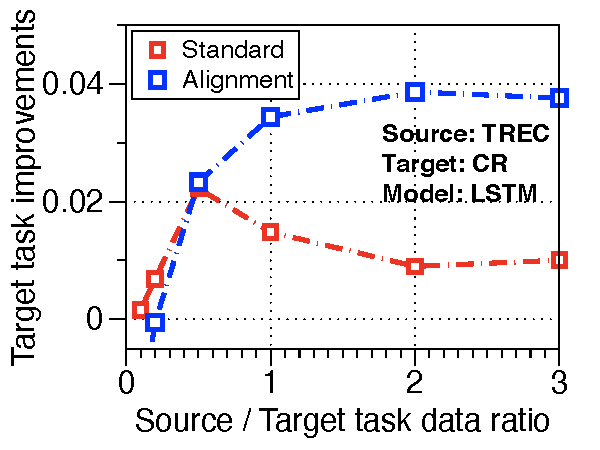
\includegraphics[width=0.975\textwidth]{figures/ratio_alignment_norm_trec_cr_lstm.pdf}
		\caption{Task pair TREC and CR}
	\end{subfigure}\hfill
		\begin{subfigure}[b]{0.33\textwidth}
		\centering
		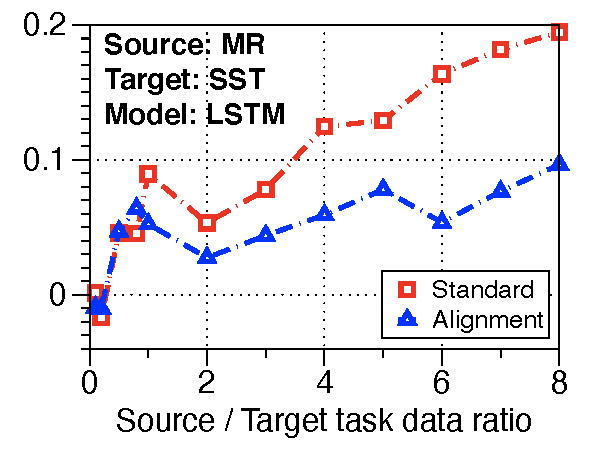
\includegraphics[width=0.975\textwidth]{figures/ratio_alignment_mr_sst_lstm.pdf}
		\caption{Task pair MR and SST}
	\end{subfigure}
	\caption{The performance of aligning task covariances depends on data size. As the ratio between source task data size and target task data size increases, the performance improvement from aligning task covariances increases.}
	\label{fig_covariate_app}
\end{figure}


\textbf{Task similarity.} We validate that MTL performs better when the source task is more similar to the target task.
We show the result on the sentiment analysis tasks.
For a target task, we manually select a similar task and a dissimilar task based on prior knowledge.
Figure \ref{fig_ab_sim} confirms the result.
Recall that Section \ref{sec_data_size} shows that increasing the data size of the source task does not always improve the performance of MTL for the target task.
In Figure \ref{fig_ab_data}, we show that for source task MR and target task SST, there is a transition from positive to negative transfer as we increase the data size of the source task.
%Our result provides a fine-grained insight on the covariance alignment algorithm proposed in \cite{WZR20}.
%Recall that the covariance alignment procedure in \cite{WZR20} adds an additional module between the word embedding representation and the shared module.
When the source task data size is particularly large compared to the target task, we show that applying the covariance alignment algorithm results in more significant gains.
In Figure \ref{fig_ab_cov}, we observe that the benefit from aligning task covariances becomes more significant for LSTM and MLP as we increase the number of datapoints of the source task.

\footnote{http://nlp.stanford.edu/data/wordvecs/glove.6B.zip}
